\documentclass[11pt]{article}

\usepackage[in]{fullpage}

\usepackage{times}
\usepackage[rflt]{floatflt}
\usepackage{epsfig,subfigure,wrapfig,color,graphicx,picture}
\usepackage{amsmath,amscd,amssymb,algorithm,algorithmic,theorem,float,bbm,bm,enumerate}
\usepackage{hyperref}


\setlength{\topmargin}{-1in}
\addtolength{\topmargin}{2.5cm}

\setlength{\headheight}{0in}
\setlength{\headsep}{0in}
%\setlength{\footskip}{0in}

\setlength{\parindent}{0mm}
\setlength{\parskip}{3mm}

\setlength{\textheight}{11in}
\addtolength{\textheight}{-4.8cm}


\newcommand{\HRule}{\rule{\linewidth}{0.5mm}}

% next two lines are for \mathbbold{1}
\DeclareSymbolFont{bbold}{U}{bbold}{m}{n}
\DeclareSymbolFontAlphabet{\mathbbold}{bbold}

\begin{document}

\HRule
\begin{center}
\begin{minipage}{0.5\textwidth}
\begin{flushleft} \large
\emph{CSci 5525 (Fall'12): Machine Learning}
\end{flushleft}
\end{minipage}
\hspace*{13mm}
\begin{minipage}{0.4\textwidth}
\begin{flushright} \large
\emph{Lecture: 22 (Nov 19)}
\end{flushright}
\end{minipage}
\vspace*{5mm}

{\LARGE Expectation Maximization}\\
\vspace*{5mm}

\begin{minipage}{0.4\textwidth}
\begin{flushleft} \large
\emph{Lecturer:}\\ 
Arindam Banerjee
\end{flushleft}
\end{minipage}
\hspace*{25mm}
\begin{minipage}{0.4\textwidth}
\begin{flushright} \large
\emph{Scribe:} \\
James Benhardus\\
Joshua Lynch\\
Michael Powell
\end{flushright}
\end{minipage}

\end{center}
\HRule\\

\section{Expectation Maximization}

%review: Gaussian Mixtures Revisited
We began by recalling that for Gaussian mixtures, the EM algorithm involves an E-step of evaluating the probabilities 
\begin{align*}
p(z_{k}|x_{n}) = \frac{\pi_{k}\mathcal{N}(x|\mu_{k},\Sigma_{k})}{\sum_{j=1}^{K}\pi_{j}\mathcal{N}(x|\mu_{j},\Sigma_j)}
\end{align*}
and the M-step computes the new parameters 
\begin{align*}
\mu_k &= \frac{1}{N_{k}}\sum_{n=1}^{N}{p(z_{k}|x_{n})x_{n}} \\
\Sigma_{k} &= \frac{1}{N_{k}}\sum_{n=1}^{N}{p(z_{k}|x_{n})(x_{n}-\mu_{k})(x_{n}-\mu_{k})^{T}} \\
\pi_{k} &= \frac{N_{k}}{N}
\end{align*}

We then turned our attention to why the EM algorithm works.  

EM is applicable when there is missing information.  For example, in clustering missing information is: what cluster does each data point belong to?  Call this missing information (cluster for each data point) $Z$, and call the data points themselves $X$.  If we are fitting Gaussian mixture models then we are also missing the parameters ${\mu_k}, {\Sigma_k}$.  The EM algorithm proceeds by guessing $Z$, finding $\mu_k, \Sigma_k$, updating $Z$, updating $\mu_k, \Sigma_k$, and repeating until convergence.

In general, for a probabilistic model one can write the log likelihood as

\begin{align*}
\log p(X|\theta) &= \mathcal{L}(q,\theta) + KL(q||p) \\
                           &= E_{q(Z)}[\log p(X,Z|\theta)] + H(q) + KL(q||p)
\end{align*}

where

\begin{align*}
\mathcal{L}(q,\theta) &= \sum_{z}{q(Z)\log(\frac{p(X,Z|\theta)}{q(Z)})} \\
KL(q||p) &= \sum_{z}{q(Z)\log(\frac{q(Z)}{p(Z|X,\theta)})}
\end{align*}

But we can not maximize $p(X|\theta)$ directly because we do not know $\theta$.  Since $ KL(q||p) \geq 0$, this means that we have a lower bound on the log-likelihood of

\begin{align*}
\log p(X|\theta) &\geq \mathcal{L}(q,\theta) = E_{q}[\log p(X|\theta)] + H(q)
\end{align*}

In the E-step, maximize $\mathcal{L}(q,\theta)$ with respect to $q$.  Since $\log(p(X|\theta))$ does not depend on $q$ we can focus on minimizing the KL divergence $KL(q||p)$. If we use $q(Z) = p(Z|X,\theta)$ as our solution, we have $KL(q||p) = 0$ so for our current parameter estimate $\log p(X|\theta) = \mathcal{L}(q,\theta)$. In the M-step, we maximize $\mathcal{L}(q,\theta)$ with respect to $\theta$. This gives us a new estimated parameter $\theta^{new}$ where for our current $q$, $\mathcal{L}(q,\theta^{new}) \geq \mathcal{L}(q,\theta)$.  However, since the current q is not the optimal distribution for $\theta^{new}$, $KL(q||p) \geq 0$. This means that 

\begin{align*}
\log p(X|\theta^{new}) &\geq \mathcal{L}(q,\theta^{new}) \geq \mathcal{L}(q,\theta) = \log p(X|\theta)
\end{align*}

So the log-likelihood will either increase or stay the same after each combination of E-step and M-step.

Variational EM

Over the past 10 years a very popular variant of the EM algorithm has been Variational EM, especially for statistical models.  For some models $p(Z|X,\theta)$ cannot be obtained in closed form.  In this case pick a parameterized family $q_{\gamma}=q(Z|\gamma)$ and minimize with respect to $\gamma$ to minimize $KL(q_{\gamma}||p)$.  This is the same as maximizing a lower bound to the true likelihood

\begin{align*}
\log p(X|\theta) \geq E_{q_{\gamma}}[\log p(X,Z|\theta)] + H(q_{\gamma})
\end{align*}

In this process, $KL(q_{gamma}||p)$ does not become zero, but it does decrease.

Auxillary Function Viewpoint of EM

Here is another viewpoint on EM.  If we want to optimize an objective function $f$ or parameters of a model but we can not do gradient descent because of missing information, then we can use EM.  The EM algorithm constructs a simple 'surrogate' convex function $g$ that agrees with the objective function at some $\theta^{old}$ and is everywhere else less than the objective.  Then the value $\theta^{new}$ which maximizes the surrogate function is found.  We know $f(\theta^{new}) \ge f(\theta^{old}) \ge g(\theta^{old}) = f(\theta^{old})$ by construction.  Now we can construct a new convexfunction $h$ that agrees with $f$ at $\theta^{new}$ but is otherwise always less than or equal to $f$.

A Final Point

One last thing about learning mixture models.  Over the last 15 years there have been interesting developments in computer science for learning mixture models that do not use EM, which may get stuck in bad local minima.  These new methods give better guarantees and are theoretically elegant but are difficult to implement.

\section{Spectral Clustering}
Spectral clustering is a method of assigning data objects to different clusters or classes.  It differes from K-means clustering in that it does not necessarily rely on any Euclidean distance metric and does not make any implicit assumptions about the shape of the clusters within the overall dataset.

The first step in spectral clustering is to create an undirected, weighted graph G among the n data objects under study.  The graph consists of vertices $V=\{v_i:1,2,\dots,n\}$ and edges $E=\{e_{ij}:v_i, v_j \text{ are adjacent}\}$.  The vertices represent the n data objects, which can be anything and do not need to be vectors.  The edges connect vertices that are 'similar' according to any measure of similarity the researcher chooses.  Here is an example of a simple graph representing 7 data objects of some sort:

\begin{figure}
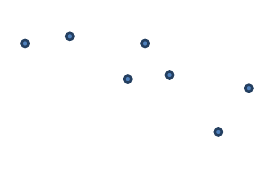
\includegraphics{graph_0}
\caption{}
\end{figure}

Each edge $e_{ij}$ will have a weight $w_{ij}$ representing the degree of similarity between the two vertices (the absence of an edge represents a weight of 0).  These weights can be arranged as a matrix $[w_{ij}]$.

Here is the weight matrix corresponding to the example graph above (assuming for simplicity that all edges in the graph have a weight of 1):

Then, the degree $d_i$ of each vertex is calculated.  For a given node, the degree of that node is a measure of its connectivity wth other nodes.  In a weighted graph, the degree is the sum of the weights between a node and all the other nodes it is connected to.  The degrees $d_i$ of all the vertices can be arranged in a diagonal matrix.


%(slide: graph cuts and spectral clustering)
Consider a data set like (***    ****) and another like (a smiley face).  The second data set is not handled well by k-means because a certain geometric structure is assumed.

%(slides: example data set slides)

%(slide: similarity graphs)
G=(V,E) a weighted, undirected graph; assume we have already constructed the graph.
Each vertex is a data point; a data point need not be a real-valued vector ($x \in \mathbb{R}^d)$.
The edge weight tells how similar are 2 data points.

%(slide: graph notation)
\begin{align*}
\text{deg}(i) &=\sum w_{ij} \\
\text{'cut'} \bar{A} &=V \ A \\
\mathbbold{1}_A &= \begin{bmatrix}
 1 \\
 1 \\
 0 \\
 0
\end{bmatrix}
\end{align*}

%(slide: unnormalized graph Laplacian)
The unnormalized graph Laplacian is the 'first' kind of graph Laplacian:
\begin{align}
L_U = D - W
\end{align}
where D is a diagonal matrix of vertex degrees and W is the weight matrix (adjacency matrix).  Note diagonal of W is zero since no self-connections.  Also note the sum of each row of $L_U$ is zero.

What's special about $L_U$?
For any $f \in \mathbb{R}^n$, 

\begin{align}
f^TL_Uf=\sum_{i,j}w_{ij}(f_i-f_j)^2
\end{align}
is convex if $L_U$ is positive semidefinite.  In fact, $L_U$ is always symmetric and positive semidefinite.  What does the RHS tell us?  (figure *v*---*x*) To minimize $f^TL_Uf$ we need $f_i=f_j$ for edges with large weight.  Edges with low weight can have different $f_i,f_j$.  This is at the crux of what spectral clustering algorithms try to do.  The smallest eigenvalue of $L_U$ is 0, this is the 'trivial solution' for clustering.  The corresponding eigenvector is $\mathbbold{1}$.  Since $L_U\mathbbold{1}=0$ since $L_U\mathbbold{1}$ is a column of row sums.  This may not be so exciting.  Here's the exciting part:

%(slide: A Key Property)
Number of 0 eigenvalues is number of connected components.  (figure: smiley face)
%% Add your references to myrefs.bib and uncomment the following 2 lines
%\bibliography{myrefs}
%\bibliographystyle{plain}

\end{document}
